\chapter{Issues and Future Work}


\section{Issues} 
One of the design issues faced during the development is where should the SDK be installed from Architecture point of view?
1-On the server side where the hyperledger fabric lives?  or 2-On the Client side (Android side) taking into consideration there is no official support for an Android SDK. The only supported SDKs are on GO, javascript, and java.
We implemented the SDK on the server side where Hyperledger fabric lives, thus we are obscuring the network and only exposing the node.js App with all scripts that consume the request and make SDK calls to interact with the ledger designing the backend that way by totally obscuring the hyperledger fabric network will have the following advantages: 

\begin{enumerate}
  \item Since there is no officially supported SDK for Android it will require much time and effort to redevelop an Android SDK, as there is no point for reinventing the wheel. 
  \item Abstract the client and the knowledge of hyperledger fabric. assume we wanted to scale our application and develop a web site or an ios version the developer will have to dedicate so many hours to integrate the SDK in addition he must be aware of hyperledger fabric, instead of just using a simple network call without knowing what is behind the network.    
  \item Standardizing the communication using APIs. this way all the APIs could be easily standardized and manifested   
  \item Avoiding the latency and restricting all the transaction flow on the internal network. so the communication between the SDK and the peers will be done on the internal network and we avoid the delay will be introduced if the request was made on the internet with many hobs
  \item The communication will be encrypted using SSL certificate. All the header and payload will be encrypted.
  \item The Whole hyperledger fabric network will be isolated and couldn't be directly accessed from the internet in case of the web server compromised the data and all the network will be safe. 
  \item Finally, Avoiding the unnecessary SDK Library size on the smartphone. 
\end{enumerate}
\clearpage
\noindent One main disadvantage of this approach is the data could be viewed by the server admin, However, to modify the data directly will be nontrivial and could be easily investigated.  since the data on the ledger is append-only and the business logic is reinforced by the chaincode. Furthermore introducing a simple cryptographic scheme to cipher the data would resolve this issue. 
\hyperref[fig:enrollmentproc]{Figure 5.1} depicts how the network is obscured.  
\ \\
 \begin{figure}[H]
\center
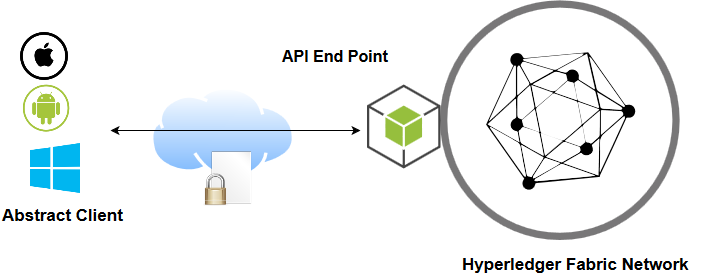
\includegraphics[width=10cm,height=8cm]{images/issues.png}
\caption{Obscuring the Network by Using the Node.js App }
\label{fig:issues}
\end{figure}

\section{Future Work} 

Based on our reusable and modular design we could adopt any complex business logic by simply modifying the chaincode. Furthermore, we could introduce more roles such as, Researchers and verifiers who could have more privileges like banning other users who scam the platform and prevent any malicious behavior. 
 
